%%=============================================================================
%% Conclusie
%%=============================================================================

\chapter{Conclusie}
\label{ch:conclusie}

% TODO: Trek een duidelijke conclusie, in de vorm van een antwoord op de
% onderzoeksvra(a)g(en). Wat was jouw bijdrage aan het onderzoeksdomein en
% hoe biedt dit meerwaarde aan het vakgebied/doelgroep? 
% Reflecteer kritisch over het resultaat. In Engelse teksten wordt deze sectie
% ``Discussion'' genoemd. Had je deze uitkomst verwacht? Zijn er zaken die nog
% niet duidelijk zijn?
% Heeft het onderzoek geleid tot nieuwe vragen die uitnodigen tot verder 
%onderzoek?

De opzet van dit onderzoek is om een antwoord te geven op de onderzoeksvragen “Welk dataformaat is performanter voor de Discovery API van de Fashion Society?”, “Is gRPC met ProtocolBuffers sneller dan REST API met JSON voor de implementatie van de Fashion Society?” en “Is gRPC met ProtocolBuffers efficiënter dan REST API met JSON op gebied van CPU gebruik voor de implementatie van de Fashion Society?”.
De conclusie is afhankelijk van de drie uitgevoerde testen, single call response time, totale response tijd voor vierduizend parallelle calls en totale response tijd voor tienduizend parallelle calls, die voor de methode GetService en GetServiceUrl zijn uitgevoerd.

\section{Single Call}
\label{sec:Single Call}
Uit het onderzoek is gebleken dat gRPC met ProtocolBuffers voor zowel de GetService methode (-24,06\%) als de GetServiceUrl methode (-23,78\%) sneller is dan REST met JSON.
\begin{figure}[H]
    \centering
    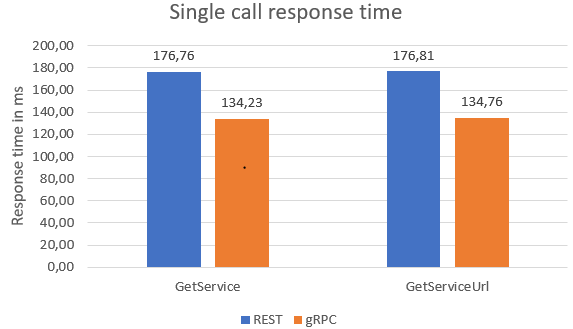
\includegraphics[scale=1]{singleCall}
    \caption[Single Call Response Time]{Resultaat van het onderzoek naar Single call response time.}
    \label{fig:SingleCallResult}
\end{figure}

De verwachting van dit onderdeel was dat het resultaat bij de single call response time een marginaal verschil ging zijn in voordeel van gRPC doordat de response op de calls een kleine hoeveelheid data is voor beide methodes, echter toonde het resultaat een groter dan verwacht verschil in snelheid in voordeel  van gRPC.

\section{Vierduizend Parallelle Calls}
\label{sec:Vierduizend parallelle calls}
Uit het onderzoek is gebleken dat gRPC voor zowel de GetService methode (-15,63\%) als voor de GetServiceUrl methode (-20,34\%) sneller is dan REST bij het afhandelen van vierduizend parallelle calls.
\begin{figure}[H]
    \centering
    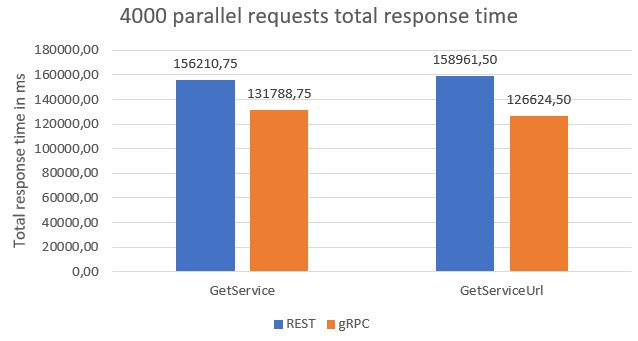
\includegraphics[scale=1]{VierduizendCalls}
    \caption[Resultaten van vierduizend parallelle calls]{Resultaat van het onderzoek naar een kleine hoeveelheid parallelle calls.}
    \label{fig:VierduizendCallsResult}
\end{figure}

Bij dit onderdeel is het resultaat onder de verwachtingen, de verwachtingen waren dat gRPC opmerkelijk sneller ging zijn dan REST door de hoeveelheid aan af te handelen requests. Echter is het gebleken dat dit een verkeerde redenering was voor de verwachting, de hoeveelheid data in de response op elke call blijft namelijk nog altijd klein.

\section{Tienduizend Parallelle Calls}
\label{sec:Tienduizend parallelle calls}
Uit het onderzoek is gebleken dat gRPC voor zowel de GetService methode (-13,96\%) als voor de GetServiceUrl methode (-16,35\%) sneller is dan REST bij het afhandelen van tienduizend parallelle calls.
\begin{figure}[H]
    \centering
    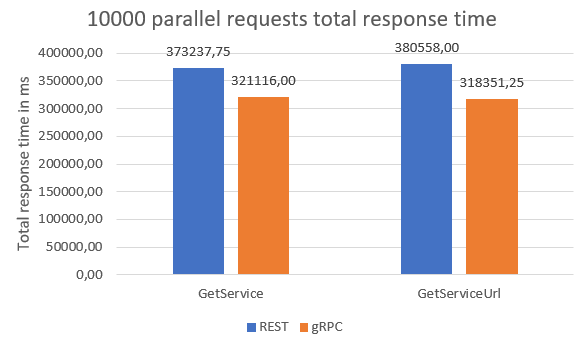
\includegraphics[scale=1]{TienduizendCalls}
    \caption[Resultaten van tienduizend parallelle calls]{Resultaat van het onderzoek naar een grote hoeveelheid parallelle calls.}
    \label{fig:TienduizendCallsResult}
\end{figure}

Net zoals bij de kleine hoeveelheid parallelle calls is het resultaat hier onder de verwachtingen. gRPC is voor zowel de GetService methode (-13,96\%) als voor de GetServiceUrl methode (-16,35\%) sneller dan REST maar ook hier is voor de verwachting dezelfde verkeerde redenering gebruikt als bij de kleine hoeveelheid parallelle calls. Het aantal parallelle calls is wel verhoogd maar de hoeveelheid data in de response op de calls blijft nog altijd hetzelfde.

\section{Besluit}
\label{sec:Besluit}

Uit het onderzoek kunnen twee van de drie onderzoeksvragen beantwoord worden. Er kan geconcludeerd worden dat gRPC met ProtocolBuffers sneller is dan REST met JSON voor de implementatie van The Fasion Society en dat ProtocolBuffers performanter zijn dan JSON voor de implementatie van de Fashion Society.

Op de onderzoeksvraag “Is gRPC met ProtocolBuffers efficiënter dan REST API met JSON op gebied van CPU gebruik voor de implementatie van de Fashion Society?” kan geen besluitend antwoord gegeven worden omdat deze gegevens niet exact meetbaar waren gedurende het uitvoeren van de proof-of-concept. Hierbij is in overleg met de co-promotor het besluit gevormd dat de Fashion Society een snel groeiend bedrijf is waarbij performantie belangrijk is en dat als er meer CPU gebruik zou zijn dit een prijs is dat het bedrijf gewillig is om te betalen in ruil voor een performantere implementatie.





